
\chapter{Содержание}

\textit{Цель работы}:  построение доверительных интервалов для математического ожидания и дисперсии нормальной случайной величины
\begin{enumerate}[wide=0pt]
	\item Для выборки объема n из генеральной совокупности X реализовать в виде программы на ЭВМ:
	\begin{enumerate}
		\item вычисление точечных оценок $\hat\mu(\vec X_n)$ и $S^2(\vec X_n)$ математического ожидания $MX$ и дисперсии $DX$ соответственно;
		\item вычисление нижней и верхней границ $\underline\mu(\vec X_n)$, $\overline\mu(\vec X_n)$ для $\gamma$-доверительного интервала для математического ожидания $MX$;
		\item вычисление оценок $\hat{\mu}$ и $S^2$ математического ожидания MX и дисперсии DX;
		\item вычисление нижней и верхней границ $\underline\sigma^2(\vec X_n)$, $\overline\sigma^2(\vec X_n)$ для $\gamma$-доверительного интервала для дисперсии $DX$;
	\end{enumerate}
	\item вычислить $\hat\mu$ и $S^2$ для выборки из индивидуального варианта;
	\item для заданного пользователем уровня доверия $\gamma$ и $N$ – объёма выборки из индивидуального варианта:
	\begin{enumerate}
		\item на координатной плоскости $Oyn$ построить прямую $y = \hat\mu(\vec{x_N})$, также графики функций $y = \hat\mu(\vec x_n)$, $y = \underline\mu(\vec x_n)$ и $y = \overline\mu(\vec x_n)$ как функций объема $n$ выборки, где $n$ изменяется от 1 до $N$;
		\item на другой координатной плоскости $Ozn$ построить прямую $z = S^2(\vec{x_N})$, также графики функций $z = S^2(\vec x_n)$, $z = \underline\sigma^2(\vec x_n)$ и $z = \overline\sigma^2(\vec x_n)$ как функций объема $n$ выборки, где $n$ изменяется от 1 до $N$.
	\end{enumerate}
\end{enumerate}

\chapter{Теоретические сведения}
Дана случайная величина X, закон распределения которой известен с точностью до неизвестного параметра $\theta$. 

Интервальной оценкой с коэффициентом доверия $\gamma$ ($\gamma$-доверительной интервальной оценкой) параметра $\theta$ называют пару статистик $\underline{\theta}(\vec X), \overline{\theta}(\vec X)$ таких, что

$$P\{\underline{\theta}(\vec X)< \theta< \overline{\theta}(\vec X)\}=\gamma$$ 

Формулы для вычисления границ $\gamma$-доверительного интервала для математического ожидания:

\begin{equation}
	\begin{array}{cc}
		\underline\mu(\vec X_n)=\overline X - \cfrac{S(\vec X)t^{St(n-1)}_{\frac{1+\gamma}{2}}}{\sqrt{n}}\; ; & \overline\mu(\vec X_n)=\overline X + \cfrac{S(\vec X)t^{St(n-1)}_{\frac{1+\gamma}{2}}}{\sqrt{n}}
	\end{array}
\end{equation}

$\overline X$ -- точечная оценка математического ожидания;

$S^2(\vec X)$ -- точечная оценка дисперсии;

$n$ -- объем выборки;

$\gamma$ -- уровень доверия;

$t^{St(n-1)}_{\frac{1+\gamma}{2}}$ -- квантили соответствующих уровней распределения Стьюдента с n - 1 степенями свободы.

Формулы для вычисления границ $\gamma$-доверительного интервала для дисперсии:
\begin{equation}
	\begin{array}{cc}
		\underline\sigma(\vec X_n)= \cfrac{(n-1)S^2(\vec X)}{t^{\chi^2(n-1)}_{\frac{1+\gamma}{2}}};\; & \overline\sigma(\vec X_n)= \cfrac{(n-1)S^2(\vec X)}{t^{\chi^2(n-1)}_{\frac{1-\gamma}{2}}}
	\end{array}
\end{equation}

$S^2(\vec X)$ -- точечная оценка дисперсии;

$n$ -- объем выборки;

$\gamma$ -- уровень доверия;

$t^{\chi^2(n-1)}_{\frac{1+\gamma}{2}}$ -- квантили соответствующих уровней распределения $\chi^2(n-1)$ с n - 1 степенями свободы.


\chapter{Результаты расчетов}
\begin{enumerate}
	\item Точечные оценки $\hat \mu (\vec x_n)$ и $ S^2 (\vec x_n)$ математического ожидания MX и дисперсии DX соответственно: $\hat \mu (\vec x_n) = -4.758$, $ S^2 (\vec x_n) = 0.812$
	\item Вычисление нижней и верхней границ $\underline \mu (\vec x_n)$, 
	$\overline \mu (\vec x_n)$ для $\gamma$-доверительного интервала для математического ожидания DX: 
	$\underline \mu (\vec x_n) = -4.894$, $\overline\mu (\vec x_n) = -4.622$

	\item Вычисление нижней и верхней границ $\underline \sigma (\vec x_n)$, 
	$\overline \sigma (\vec x_n)$ для $\gamma$-доверительного интервала для математического ожидания MX: 
	$\underline \sigma (\vec x_n) = 0.664$, $\overline \sigma (\vec x_n) = 1.019$
\end{enumerate}

\begin{figure}[ht!]
		\centering
		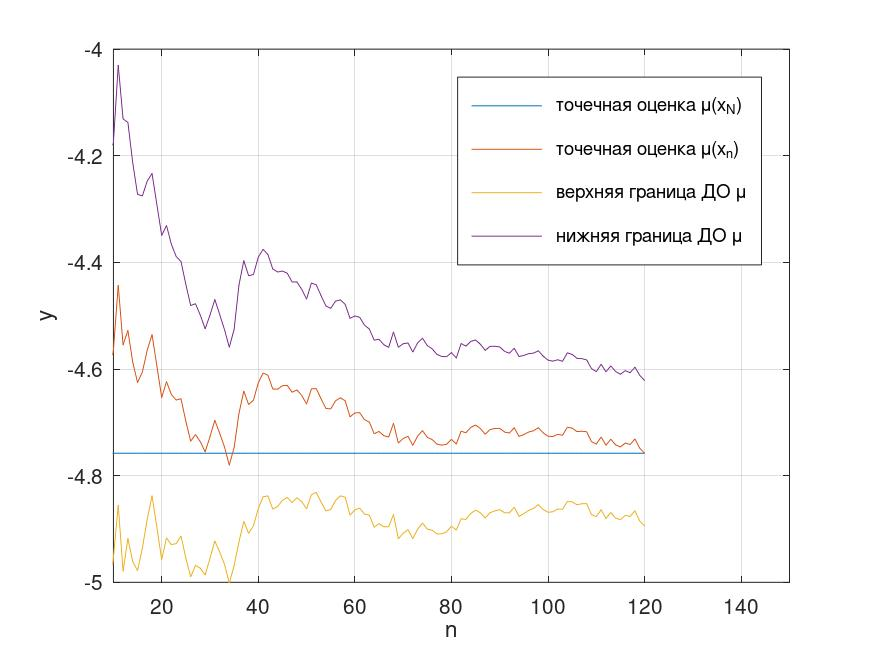
\includegraphics[scale=0.4]{assets/g-1.jpg}
		\caption{Прямая $y=\hat \mu (\vec x_N)$ и графики функций $y=\hat \mu (\vec x_n), y= \underline \mu (\vec x_n), y =\overline \mu (\vec x_n)$ как функций объема n выборки, где n изменяется от 1 до N.}
\end{figure}

\begin{figure}[ht!]
	\centering
	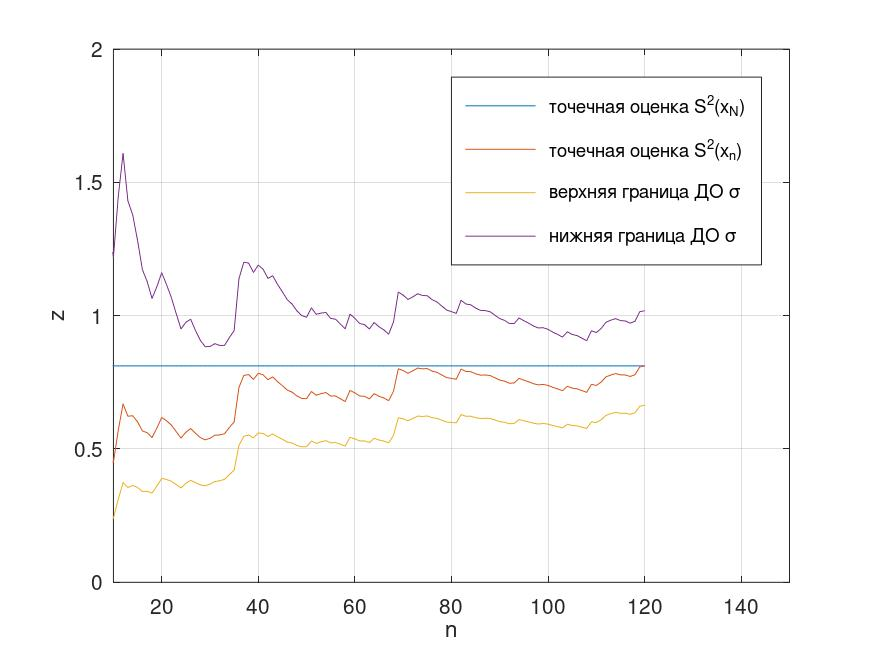
\includegraphics[scale=0.4]{assets/g-2.jpg}
	\caption{Прямая $z=\hat S^2 (\vec x_N)$ и графики функций $z= S^2 (\vec x_n), z= \underline \sigma^2 (\vec x_n), z =\overline \sigma^2 (\vec x_n)$ как функций объема n выборки, где n изменяется от 1 до N.}
\end{figure}